% Created 2021-11-25 qui 02:05
% Intended LaTeX compiler: pdflatex
\documentclass[article, a4paper, oneside, 11pt, english, brazil, sumario=tradicional]{abntex2}
		  \usepackage{times}
\usepackage[utf8x]{inputenc}
\usepackage[T1]{fontenc}
\usepackage{titlesec}
\usepackage[english, hyperpageref]{backref}
\usepackage{hyperref}
\usepackage{indentfirst}
\usepackage{titling}
\usepackage{graphicx}
\ifthenelse{\equal{\ABNTEXisarticle}{true}}{%
\renewcommand{\maketitlehookb}{}
}{}
\titleformat{\section}{\normalfont\normalsize\bfseries\uppercase}{\thesection\space\space}{0pt}{}
\titleformat{\subsection}{\normalfont\normalsize\bfseries}{\thesubsection\space\space}{0pt}{\space}
\titleformat{\subsubsection}{\normalfont\normalsize\bfseries}{\thesubsubsection\space\space}{0pt}{\space}
\titleformat{\paragraph}{\normalfont\normalsize\itshape}{}{0pt}{\theparagraph\space\space}
\setlength{\parindent}{1.5cm}
\setlrmarginsandblock{3cm}{2cm}{*}
\setulmarginsandblock{2.5cm}{2.5cm}{*}
\checkandfixthelayout



\usepackage{minted}
\author{Lucas Samuel Vieira}
\date{\today}
\title{EVA 2}
\hypersetup{
 pdfauthor={Lucas Samuel Vieira},
 pdftitle={EVA 2},
 pdfkeywords={},
 pdfsubject={},
 pdfcreator={Emacs 27.2 (Org mode 9.4.5)}, 
 pdflang={Brazilian}}
\begin{document}

\OnehalfSpacing
\pretextual
\textual

\begin{center}
\textbf{UFVJM - UNIVERSIDADE FEDERAL DOS VALES DO JEQUITINHONHA E MUCURI}

\textbf{BACHARELADO EM SISTEMAS DE INFORMAÇÃO}

\textbf{BANCO DE DADOS II - SEMESTRE 2021/1}

\textbf{Exercício de Avaliação de Aprendizagem 2 - EVA 2}
\end{center}

\noindent
Nome: Lucas Samuel Vieira
\newline

\section{Exercício 1}
\label{sec:orga00e629}

Apresente um esquema  de uma base de  dados relacional (de pelo  menos 2 tabelas
relacionadas) e descreva uma funcionalidade de  um SI que seja mapeada para mais
de uma operação SQL na base de dados. Apresente o código de uma Stored Procedure
que implemente esta funcionalidade como sendo uma transação.

\subsection{Resposta}
\label{sec:orgd3adbc1}

Para  a realização  do exercício,  será considerada  uma tabela  de venda  e uma
tabela para os itens das respectivas vendas.

O processo  de venda pode ser  visto como uma  operação a ser realizada  por uma
transação.

Para tanto, teremos uma tabela para os dados  de uma venda, e uma tabela para os
itens da mesma, como demonstrado pelas queries de criação a seguir:

\begin{minted}[]{sql}
CREATE TABLE venda (
       id INT NOT NULL AUTO_INCREMENT,
       cliente VARCHAR(50) NOT NULL,
       vendedor VARCHAR(50) NOT NULL,
       data_venda TIMESTAMP NOT NULL,
       PRIMARY KEY(id)
);

CREATE TABLE venda_itens (
       id INT NOT NULL AUTO_INCREMENT,
       descricao VARCHAR(50) NOT NULL,
       venda_id INT NOT NULL,
       PRIMARY KEY(id),
       FOREIGN KEY(venda_id) REFERENCES venda(id)
);
\end{minted}

Sendo  assim, para  realizar  uma venda,  basta que  façamos  uma transação  que
garanta que  a venda e  seus itens sejam  inseridos atomicamente, como  mostra a
procedure a seguir.

\begin{minted}[]{sql}
DELIMITER &
CREATE PROCEDURE sp_realiza_venda_teste()
BEGIN
    DECLARE venda_indice int;
    DECLARE data_atual timestamp;

    START TRANSACTION;

    SELECT CURRENT_TIMESTAMP INTO data_atual;

    INSERT INTO venda (cliente, vendedor, data_venda)
    VALUES ('Fulano da Silva', 'Vendedor da Silva', data_atual);

    SELECT LAST_INSERT_ID() INTO venda_indice;

    INSERT INTO venda_itens (descricao, venda_id)
    VALUES
        ('Shampoo', venda_indice),
        ('Condicionador', venda_indice),
        ('Sabonete', venda_indice);

    COMMIT;
END &
DELIMITER ;
\end{minted}

O resultado pode ser verificado com a query a seguir:

\begin{minted}[]{sql}
SELECT v.id, v.cliente, v.vendedor, i.descricao, v.data_venda
  FROM venda v
  JOIN venda_itens i ON v.id = i.venda_id;
\end{minted}

\section{Exercício 2}
\label{sec:orgba44280}

Apresente um esquema de uma sequência  de operações de 2 transações ocorrendo no
tempo (como foi visto em vídeo aula) que implique num deadlock (transações sobre
qualquer base de dados utilizada na disciplina).

\subsection{Resposta}
\label{sec:org8090498}

Para o exercício a seguir, foi utilizado  o banco de dados \texttt{concurso}, utilizado na
disciplina.

Para o exemplo, criaremos dois  terminais. No primeiro terminal, iniciaremos uma
transação,  e então  mudaremos  a  \texttt{descricao} do  município  de  código 2  para
\texttt{"Municipio 2"}, sem realizar \emph{commit}.

\begin{minted}[]{sql}
-- Terminal 1
START TRANSACTION;
UPDATE municipio SET descricao = 'Municipio 2'
 WHERE cod_municipio = 2;
\end{minted}

Ao mesmo tempo,  no segundo terminal, modificaremos a descrição  do município de
código 3 para \texttt{"Municipio 3"}, também em uma transação, sem realizar \emph{commit}.

\begin{minted}[]{sql}
-- Terminal 2
START TRANSACTION;
UPDATE municipio SET descricao = 'Municipio 3'
 WHERE cod_municipio = 3;
\end{minted}

Agora, no  Terminal 1, tentaremos alterar  a descrição do município  de código 3
para um  texto qualquer. Isso fará  com que o Terminal  1 entre em um  estado de
espera, aguardando o encerramento da transação no Terminal 2.

\begin{minted}[]{sql}
-- Terminal 1
UPDATE municipio SET descricao = 'Texto'
 WHERE cod_municipio = 3; -- Em espera
\end{minted}

Neste  momento, poderemos  causar um  \emph{deadlock} proposital  se, no  Terminal 2,
tentarmos  alterar  a descrição  do  município  de  código  2 para  outro  texto
qualquer.

\begin{minted}[]{sql}
-- Terminal 2
UPDATE municipio SET descricao = 'OutroTexto'
 WHERE cod_municipio = 2; -- Deadlock!
\end{minted}

Isso   causará  uma   espera  circular   entre   as  transações   de  ambos   os
terminais.  Neste   momento,  o   banco  de   dados  (mais   especificamente,  a
implementação open source  do MySQL, o MariaDB) matará a  transação causadora do
\emph{deadlock} no Terminal 2, e a query anteriormente em espera, no Terminal 1, será
realizada, ainda sem realizar \emph{commit} na transação.

A figura a seguir mostra a aplicação do exemplo em uma máquina real, com os dois
terminais conectados ao SGBD.

\begin{figure}[H]
\centering
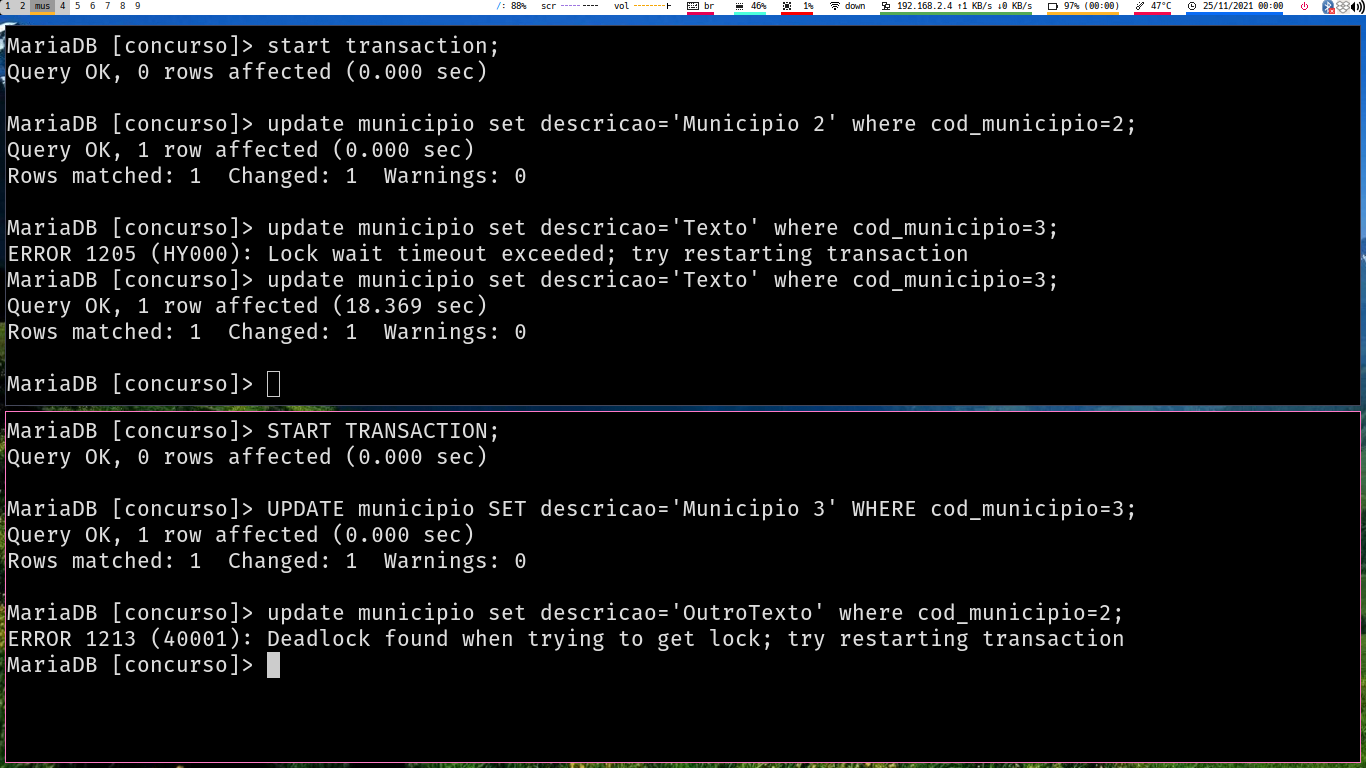
\includegraphics[width=.9\linewidth]{./deadlock.png}
\caption{Exemplo de \emph{deadlock} entre duas transações ocorrendo no MariaDB, executado via Docker.}
\end{figure}

\section{Exercício 3}
\label{sec:org0167df3}

Diferencie  os  protocolos de  recuperação  contra  falhas  baseado em  log  com
atualização imediata e adiada.

\subsection{Resposta}
\label{sec:org6af8632}

A recuperação contra  falhas baseada em log  envolve a criação de  um arquivo em
disco (o log) para registro das operações da transação, antes de sua efetivação;
somente após  o registro destas transações  em disco, as mesmas  começarão a ser
efetivadas, através de análise periódica da parte do SGBD.

Com relação à  efetivação no banco de dados, temos  as atualizações \textbf{imediata} e
\textbf{adiada}.

Para  a atualização  \textbf{adiada}, a  efetivação  das modificações  na transação  só
realmente ocorrerão  após todos os efeitos  da mesma estarem escritos  no log de
transações, que implica  necessariamente na escrita de ambos  \emph{start} e \emph{commit}
para aquela  transação. Caso não  haja \emph{commit} correspondente para  um \emph{start},
aquela transação não será efetuada, e será eliminada.

Para  a  atualização \textbf{imediata},  a  efetivação  das modificações  na  transação
ocorrem  logo  após serem  escritas  no  log, ou  seja,  para  cada operação  da
transação escrita no log, sua execução será imediata. Dessa forma, a recuperação
de erros será realizada através da restauração dos valores antigos alterados, de
acordo  com a  forma  como foram  registrados  no log.  Caso  não haja  \emph{commit}
correspondente para um \emph{start}, as modificações realizadas para aquela transação
serão desfeitas;  caso o \emph{checkpoint}  de leitura  de uma transação  se encontre
antes do \emph{commit} de uma transação, as operações da mesma serão refeitas.

\section{Exercício 4}
\label{sec:org49f5af0}

Diferencie índices secundários esparsos e densos.

\subsection{Resposta}
\label{sec:org66c6511}

Índices secundários são utilizados para  indexação de informações em tabelas que
não sejam  chaves primárias,  mas que constituam  uma informação  relevante para
pesquisa e que seja conveniente acelerar o processo de busca através da mesma.

Um índice secundário \textbf{denso} utiliza uma indexação através de uma informação que
seja  chave-candidata, ou  seja, que  não possua  repetição, o  que garante  que
o arquivo  de índice  possua a mesma  quantidade de registros  que o  arquivo de
dados.

Em contrapartida,  um índice secundário  \textbf{esparso} possui menos registros  que o
arquivo de dados,  uma vez que o atributo indexado  não seja chave-candidata, ou
seja, não possua critério de não-repetição.

\section{Exercício 5}
\label{sec:orgf5e96fe}

Descreva, com suas  palavras, os diferentes níveis de privilégios  que podem ser
concedidos ou revogados a usuários do SGBD MySQL.

\subsection{Resposta}
\label{sec:orgb596326}

Pode-se configurar os privilégios  de uso de um usuário no  SGBD MySQL de acordo
com os seguintes níveis:

\begin{itemize}
\item \textbf{Global}: Configura-se a permissão de leitura e escrita a nível do SGBD, o que
envolve acesso aos bancos de dados criados  e a criação dos mesmos, e também o
gerenciamento de usuários.
\item \textbf{Banco de dados}:  Configura-se a permissão de leitura e  escrita em bancos de
dados específicos do SGBD.
\item \textbf{Tabelas}: Configura-se a permissão de leitura  e escrita em certas tabelas de
um banco de dados.
\item \textbf{Colunas}: Configura-se a permissão de leitura  e escrita em certas colunas de
uma tabela do banco de dados.
\end{itemize}

Estes níveis podem  ser discriminados no uso dos comandos  \texttt{GRANT} e \texttt{REVOKE} do
MySQL,  não  sendo  explicitamente  descritos  como  acima  enumerado,  mas  sim
deduzidos de acordo com a forma como estes comandos são escritos.
\end{document}
